
\documentclass[tikz,border=10pt]{standalone}
\usetikzlibrary{arrows.meta, positioning, calc}

\begin{document}

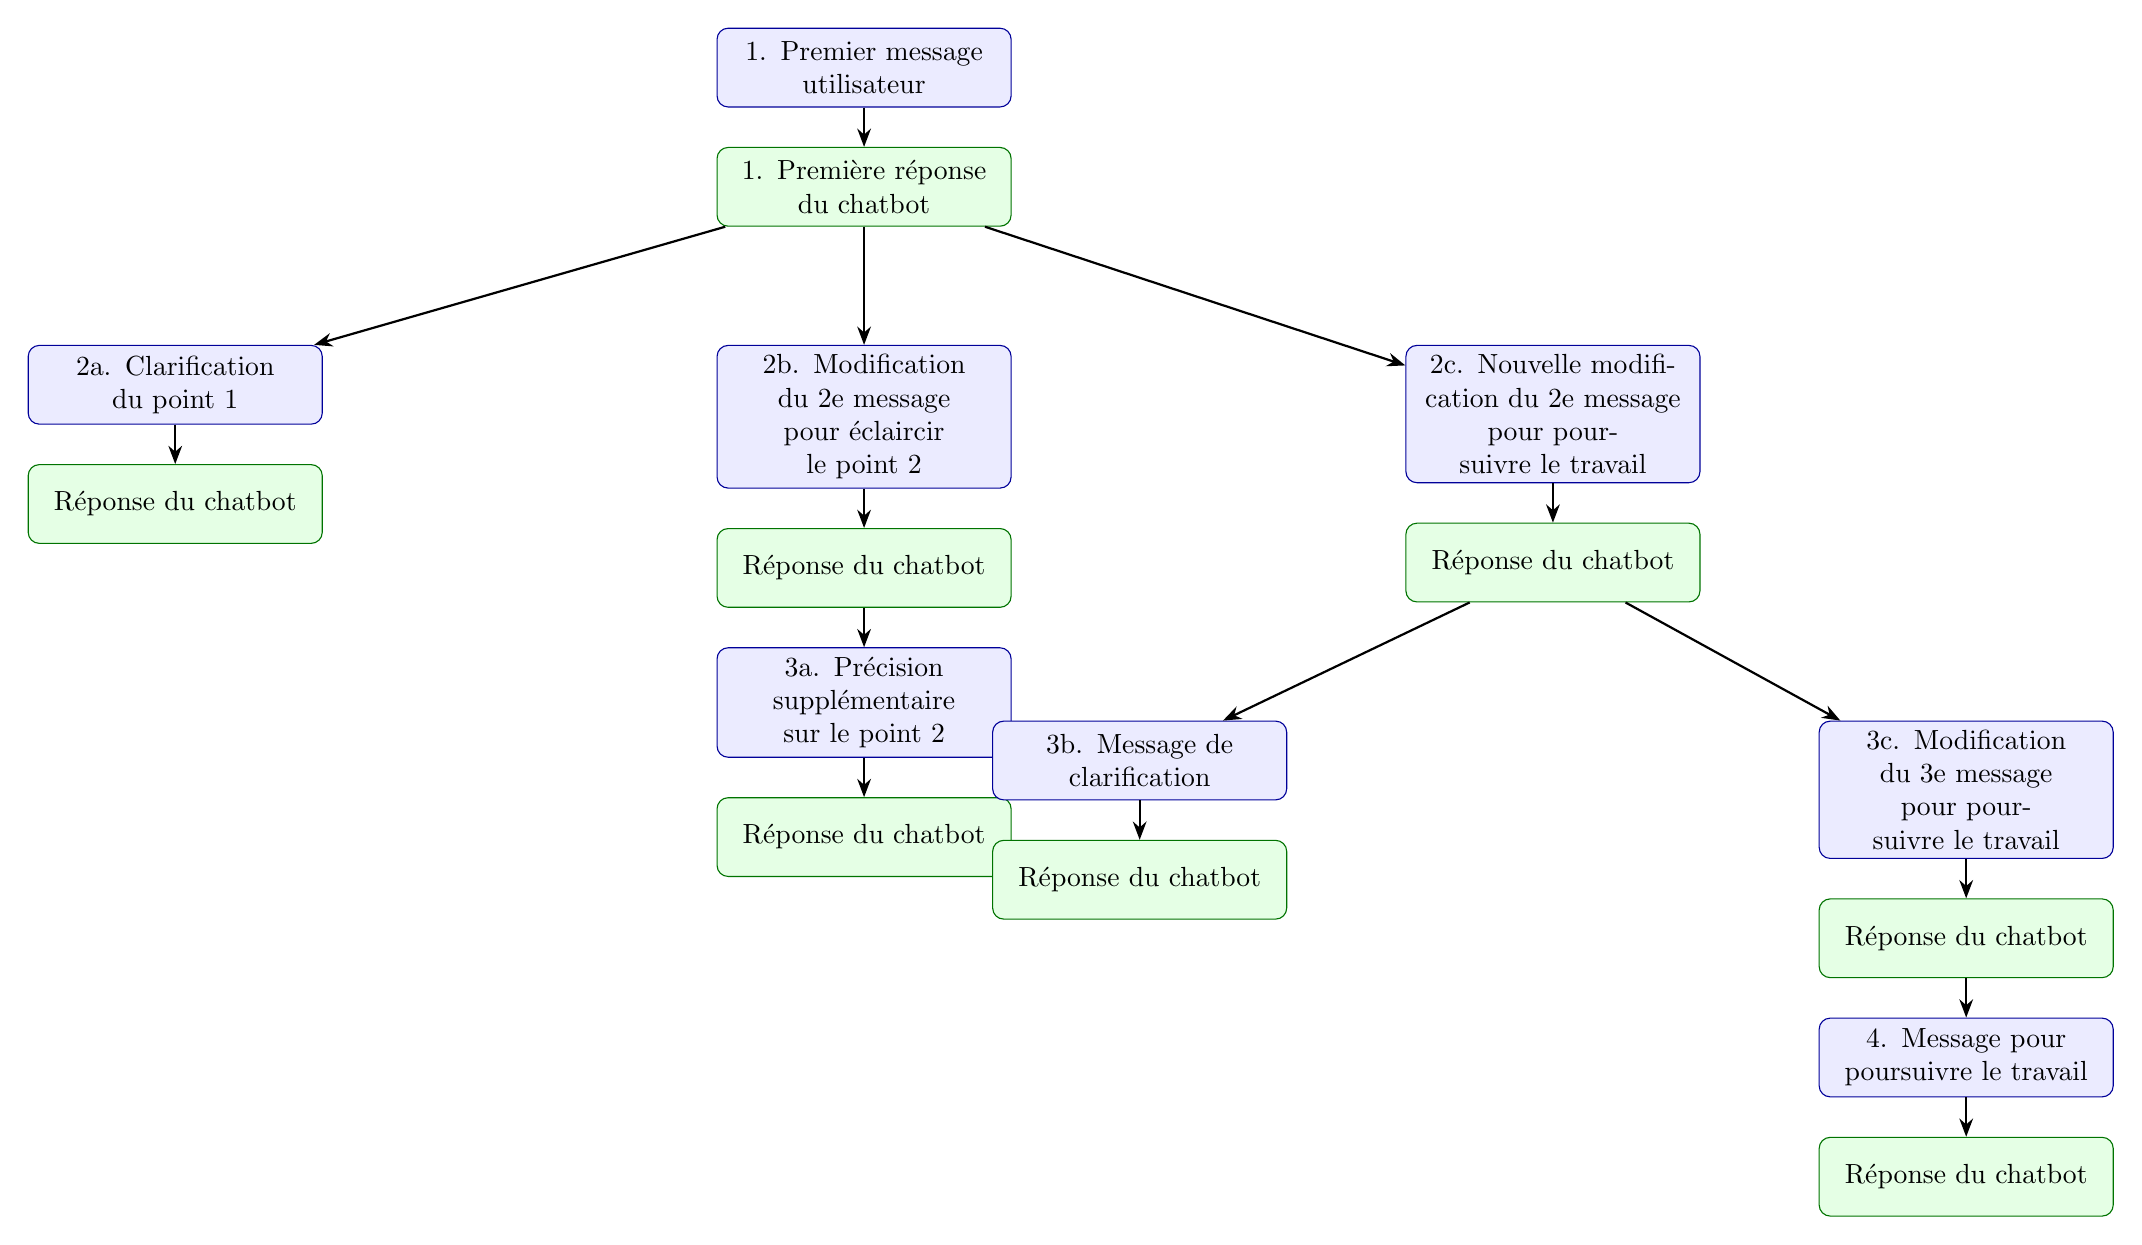
\begin{tikzpicture}[
  >=Stealth,
  user/.style={
    draw=blue!60!black,
    fill=blue!8,
    rounded corners,
    align=center,
    text width=3.5cm,
    minimum height=1cm
  },
  bot/.style={
    draw=green!45!black,
    fill=green!10,
    rounded corners,
    align=center,
    text width=3.5cm,
    minimum height=1cm
  },
  link/.style={->, thick},
  node distance=0.5cm and 1.2cm
]

% Niveau initial
\node[user] (u1) {1. Premier message\\utilisateur};
\node[bot, below=of u1] (a1) {1. Première réponse\\du chatbot};

% Niveau 2 : trois branches alignées
\node[user, below left=1.5cm and 5.0cm of a1] (u2a)
  {2a. Clarification\\du point 1};
\node[user, below=1.5cm of a1] (u2b)
  {2b. Modification du 2e message\\pour éclaircir le point 2};
\node[user, below right=1.5cm and 5.0cm of a1] (u2c)
  {2c. Nouvelle modification du 2e message\\pour poursuivre le travail};

% Réponses au niveau 2
\node[bot, below=of u2a] (a2a) {Réponse du chatbot};
\node[bot, below=of u2b] (a2b) {Réponse du chatbot};
\node[bot, below=of u2c] (a2c) {Réponse du chatbot};

% Sous-branche de 2b
\node[user, below=of a2b] (u3a)
  {3a. Précision supplémentaire\\sur le point 2};
\node[bot, below=of u3a] (a3a)
  {Réponse du chatbot};

% Sous-branches de 2c
\node[user, below left=1.5cm and 1.5cm of a2c] (u3b)
  {3b. Message de clarification};
\node[bot, below=of u3b] (a3b)
  {Réponse du chatbot};

\node[user, below right=1.5cm and 1.5cm of a2c] (u3c)
  {3c. Modification du 3e message\\pour poursuivre le travail};
\node[bot, below=of u3c] (a3c)
  {Réponse du chatbot};

% Niveau 4
\node[user, below=of a3c] (u4)
  {4. Message pour poursuivre le travail};
\node[bot, below=of u4] (a4)
  {Réponse du chatbot};

% Connexions initiales
\draw[link] (u1) -- (a1);

% Trois branches de niveau 2
\draw[link] (a1) -- (u2a);
\draw[link] (a1) -- (u2b);
\draw[link] (a1) -- (u2c);

\draw[link] (u2a) -- (a2a);
\draw[link] (u2b) -- (a2b);
\draw[link] (u2c) -- (a2c);

% Sous-branche de 2b
\draw[link] (a2b) -- (u3a);
\draw[link] (u3a) -- (a3a);

% Sous-branches de 2c
\draw[link] (a2c) -- (u3b);
\draw[link] (u3b) -- (a3b);
\draw[link] (a2c) -- (u3c);
\draw[link] (u3c) -- (a3c);

% Continuation de 3c
\draw[link] (a3c) -- (u4);
\draw[link] (u4) -- (a4);

\end{tikzpicture}
\end{document}